\documentclass[aspectratio=169, serif ]{beamer}
\usetheme{CamilaDark}

%% Fonts
\usepackage[cmintegrals,cmbraces]{newtxmath}
\usepackage{ebgaramond-maths}
\usepackage[T1]{fontenc}

\usepackage{anyfontsize}

%% Figures
\usepackage{graphicx}
\usepackage{caption}
\usepackage{subcaption}

%% Citations
\usepackage{natbib}


\title{My Title}
\subtitle{My subtitle}
\author{Me}
\institute{\texorpdfstring{ Example College\newline Example University \newline \url{example@example.com}}{}}
\date{\today}


\begin{document}

\begingroup
\setbeamertemplate{footline}{}
{
\usebackgroundtemplate{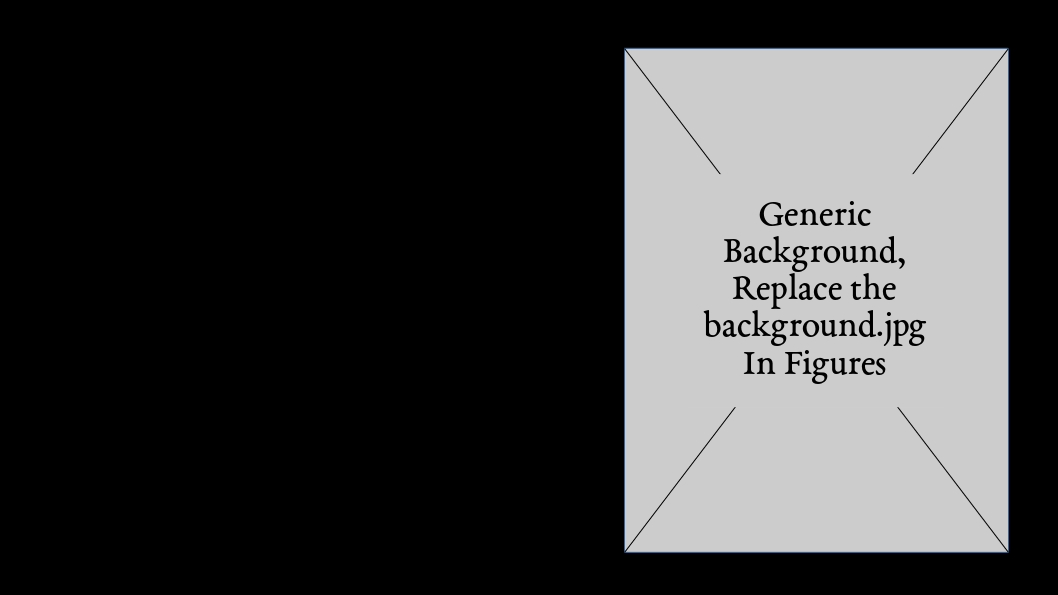
\includegraphics[width=\paperwidth]{Figures/background.jpg}}
\begin{frame}
 \titlepage
\end{frame}
}
\endgroup

\begin{frame}
    \frametitle{}
    \begin{columns}
        \column{0.4\textwidth}
            \begin{flushright}
                \textcolor{FluorescentGreen}{\huge Outline}
            \end{flushright}
        \column{0.1\textwidth}
            
        \column{0.5\textwidth}
            \tableofcontents
    \end{columns}
\end{frame}


\section{SectionOne}
\subsection{Text}
%% Frame 3

\begin{frame}
\frametitle{First slide}
    \begin{itemize}
        \item Don't be afraid to give up the good to go for the great.
        \item Doing well is the result of doing good. That's what capitalism is all about.
        \item Read more at  \url{https://www.brainyquote.com/topics/good-quotes}  
    \end{itemize}
\end{frame}

\section{SectionTwo}
\subsection{Text Bubble}
\begin{frame}{Example Text bubble}
       
    \begin{block}{Textbubble}
        \fontsize{7}{10}\selectfont
        An inexhaustible good nature is one of the most precious gifts of heaven, spreading itself like oil over the troubled sea of thought, and keeping the mind smooth and equable in the roughest weather. \newline
        
        Source: Read more at  \url{https://www.brainyquote.com/topics/good-quotes_2}
                    
    \end{block}
    
\end{frame}

\section{SectionThree}
\subsection{Tables}

\begin{frame}
    \frametitle{Tables}
    \begin{columns}
        \column{0.33\textwidth}
        \begin{table}[h]
            \centering
            \begin{tabular}{|c|c|c|c|}
                \hline
                 1& 1 & 1 & 1  \\
                 \hline
                 1& 1 & 1 & 1  \\
                 \hline
                 1& 1 & 1 & 1  \\
                 \hline
                 1& 1 & 1 & 1  \\
                 \hline
            \end{tabular}
            \end{table}
        \column{0.33\textwidth}
        \begin{table}[h]
            \centering
            \begin{tabular}{|c|c|c|c|}
                \hline
                 1& 1 & 1 & 1  \\
                 \hline
                 1& 1 & 1 & 1  \\
                 \hline
                 1& 1 & 1 & 1  \\
                 \hline
                 1& 1 & 1 & 1  \\
                 \hline
            \end{tabular}
            \end{table}
        \column{0.33\textwidth}
        \begin{table}[h]
            \centering
            \begin{tabular}{|c|c|c|c|}
                \hline
                 1& 1 & 1 & 1  \\
                 \hline
                 1& 1 & 1 & 1  \\
                 \hline
                 1& 1 & 1 & 1  \\
                 \hline
                 1& 1 & 1 & 1  \\
                 \hline
            \end{tabular}
            \end{table}
    \end{columns}
    \begin{itemize}
        \item The paterns looked for are constants biclusters with minor noise
        \item Experiments were conducted using
        \begin{itemize}
            \item Table 1 description
            \item Table 1 description
            \item Table 1 description
        \end{itemize}
    \end{itemize}
\end{frame}

\section{SectionFour}
\subsection{Figures}
\begin{frame}
    \frametitle{Figures}
    \begin{figure}
     \centering
     \begin{subfigure}[b]{0.3\textwidth}
         \centering
         
\includegraphics[width=\textwidth]{Figures/example.jpg}
         \caption{}
         \label{fig:a}
     \end{subfigure}
     \hfill
     \begin{subfigure}[b]{0.3\textwidth}
         \centering
         
\includegraphics[width=\textwidth]{Figures/example.jpg}
         \caption{}
         \label{fig:b}
     \end{subfigure}
     \hfill
     \begin{subfigure}[b]{0.3\textwidth}
         \centering
         
\includegraphics[width=\textwidth]{Figures/example.jpg}
         \caption{}
         \label{fig:c}
     \end{subfigure}
        \caption{Three simple figures}
        \label{fig:three graphs}
    \end{figure}
    Some text \ref{fig:three graphs} some text from \cite{newton1952opticks}
\end{frame}


\section{References}
\begin{frame}
 \frametitle{\textcolor{BrightYellow}{References}}
 
    \bibliographystyle{plain}
    { \fontsize{7}{10}\selectfont
    \bibliography{references}
    }
\end{frame}


\end{document}
